\chapter{Datastructure for storage of compressed volumes}  \label{ch:datastructure}

%\begin{multicols}{2}

\section{Theory}

In essence, the SVMM of a volume is generated by recursively creating copies of a lower resolution and storing them alongside each other, just like a regular MIP map. The resulting chunks of data are called the \emph{mipmap levels}, where level 0 or the \emph{base level} is the original, non-scaled volume. Where a regular mipmap level divides each side of the volume by two, SVMM can divide by an arbitrary number; this is controlled by parameter called \texttt{blockwidth} or $w$ for short.
The voxel $(x,y,z)$ at level $n+1$ is now calculated by averaging a $w^{3}$ region at level $n$ starting at $(wx,wy,wz)$. This region gives us the definition of a \emph{block} on level $n$. Subsequently, a \emph{equivalent voxel} is defined as being the single voxel on level $n+1$ that corresponds to this block on level $n$. Thus an equivalent voxel always contains the average value of all the individual voxels in the block it corresponds with.
This subdivision is repeated recursively until the resulting dimensions of a level are smaller than or equal to a certain threshold. This is parameter $r$ or the \texttt{rootwidth} and the last level is subsequently called the \emph{root level}. The root level is now the lowest resolution mipmap level generated. 

The values of $w$ and $r$ can be adapted to the size of the given volume and need to be balanced between the level of compression and the depth of the tree. Small values for $w$ would create a potentially very deep tree (note that $w=2$ generates an octree) while large values of $w$ would give almost no compression. The value for $r$ should be as large as possible as it eliminates the (needless) higher levels in the mipmap structure. However, the entire root level should still fit conveniently in memory, as we will later see. Moreover, a large $r$ obviously creates a very shallow tree and (almost) no compression can be applied.

When compared to an SVO, there are many similarities. An SVO can, for example, also be seen as an elaborate MIP Map structure. However, the fact that the SVMM datatstructure has block widths $>2$ and these widths can be selected per-level, makes it more like a $N^3$ tree rather than an octree. We deliberately avoid the term tree though, as an SVMM is conceptually closer to a collection of self-contained, multi-resolution volumes. Figure \ref{fig:svmm} gives a complete overview of the datastructure.

\begin{figure*}[b!]
\begin{center}
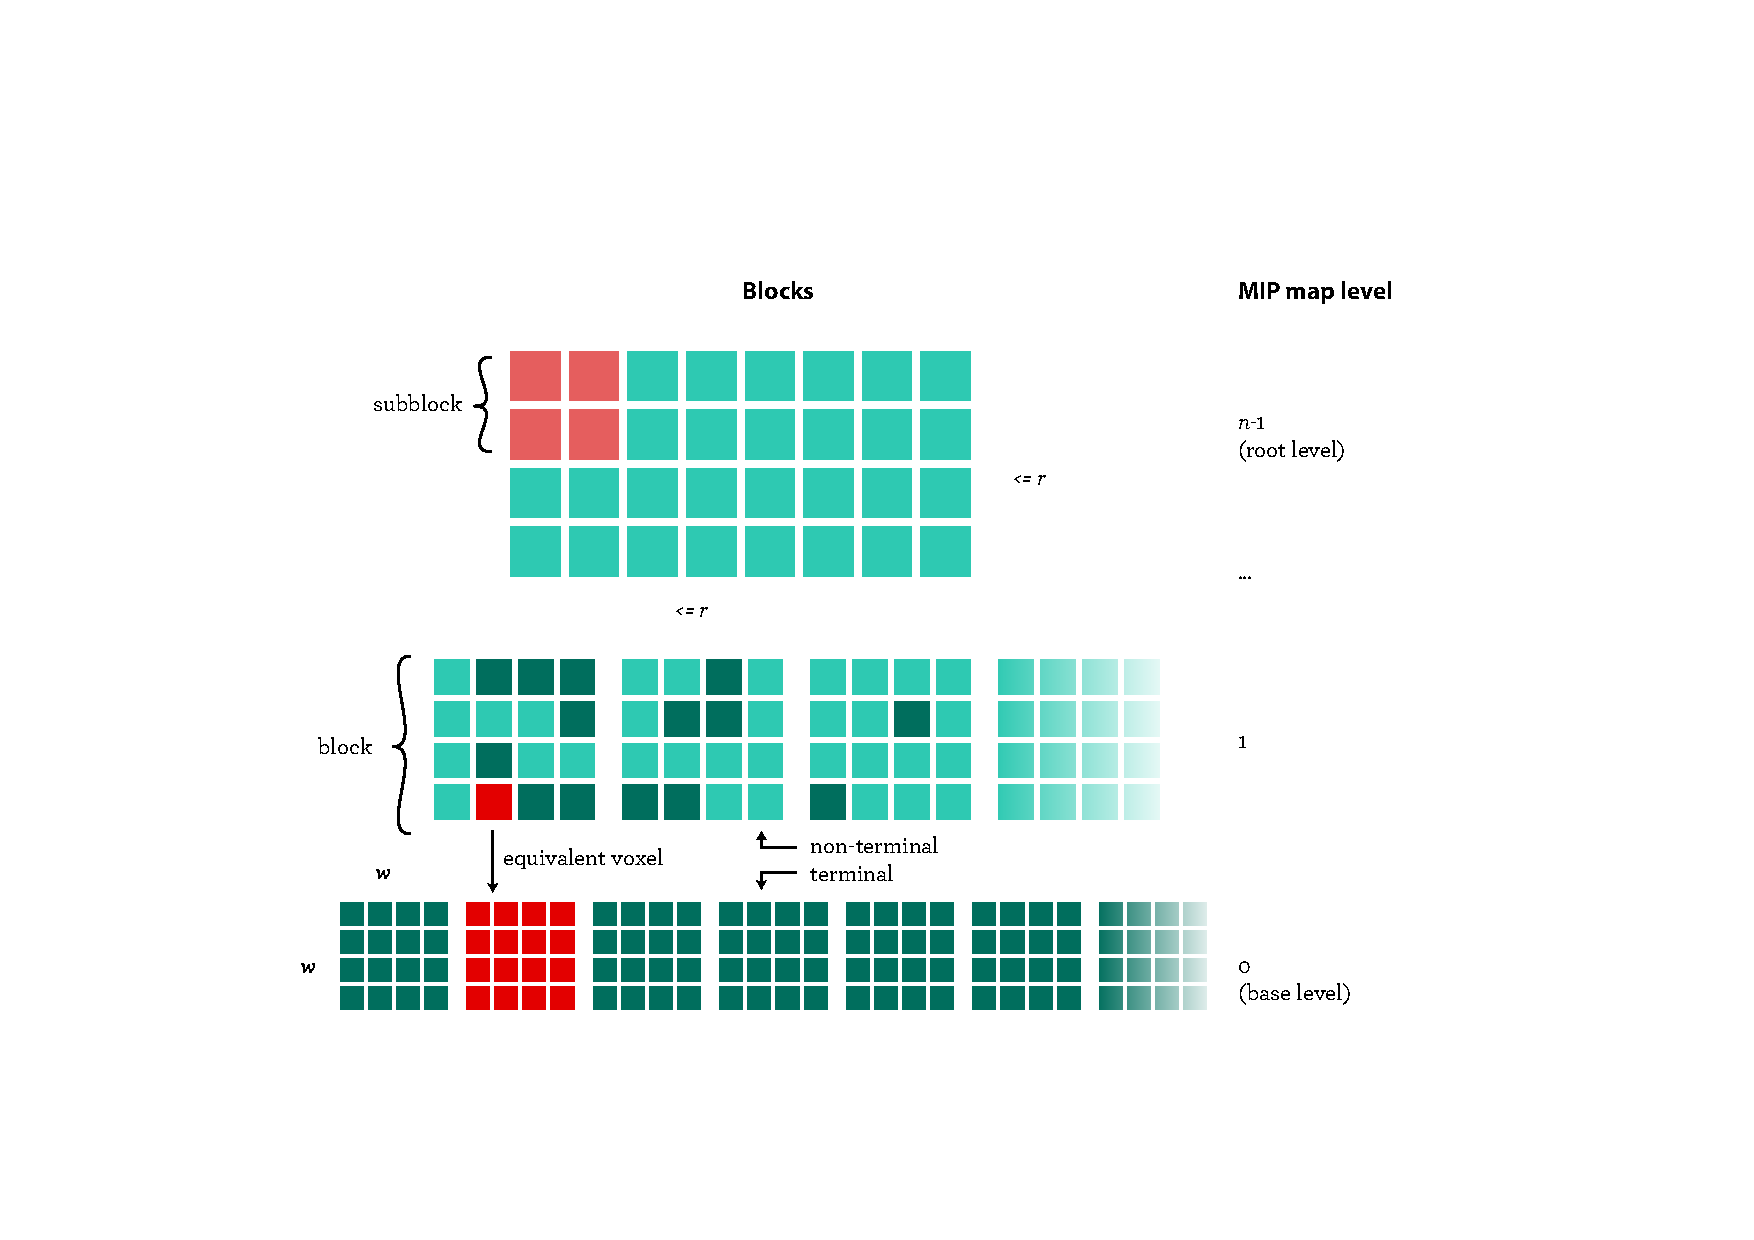
\includegraphics[scale=0.65]{figures/datastructure.pdf} 
\caption{Sparse Voxel MIP Map }
\label{fig:svmm}
\end{center}
\end{figure*}

\subsection{Compression} \label{sec:compression}

The procedure above only generates a MIP map, but does not compress the volume just yet (in fact, it adds overhead). Therefore, an extra step is added when the average of a block is calculated.
This step is designed to determine whether a certain block contributes significant information to the next mipmap level and if it does not, one could choose not to store this block. If a block is not stored, its equivalent voxel is called \emph{terminal}, i.e. no deeper mipmap levels follow. Observe that all voxels at level 0 are terminal. The resulting tree now becomes unbalanced (i.e. not all the leafs are on the same level) much like with SVOs.
When the difference between each individual voxel of a block and its equivalent voxel (the average) is smaller that a certain parameter $\delta$, it is said to be \emph{homogeneous}. If all voxels inside a homogeneous block are terminal, it may be discarded and its corresponding equivalent voxel becomes terminal. As a result, empty blocks or blocks consisting of equal voxels are not stored. 

By changing $\delta$, the amount of lossy compression that is applied can be influenced. Just like $w$ and $r$, the parameter $\delta$ can be tuned to achieve a balance between performance (image quality) and storage requirements. A large value for $\delta$ will throw out many blocks whose individual voxels are replaced by their average. This would theoretically result in a smaller memory footprint as well as a shorter rendering time (less blocks mean less traversal). The resulting volume will exhibit a `blocky' appearance much like a JPEG-compressed image.  The influence a certain value of $\delta$ has, depends on the number of attributes $n$ per voxel. Therefore, a certain intended value of $\delta$ needs to be weighted by the square root of $n$. This way, the same value of $\delta$ influences the inequality with different amounts of attributes in a similar way.
In order to handle this transparently and to improve readability, we introduce the \emph{quality factor} $q$ that ranges for 0 to 100. The quality factor directly determines $\delta$ by the equality $\delta = 1 - \sqrt{n}\frac{q}{100}$. 

Lastly, there is the option of applying additional lossy, fixed-rate (block) compression to the level-0 blocks separately. This gives an additional compression without adding complexity, and the compressed blocks can easily be stored using hardware 3D textures. The simplest method is to only store a one-bit alpha value for each voxel and discard the color information (see Figure \ref{fig:block_bitmap}). This is a bit like the chroma-luma compression commonly utilized in video. It retains all the detail of the given block, while the color information is extrapolated from its corresponding equivalent voxel. Naturally, this will degrade image quality and depending on the original volume this may or may not be acceptable. However, in it simplest form this may already give a substantial 32:1 compression ratio on the mipmap level 0 without loss of detail (assuming 32 bits are used to store one regular voxel). Of course, less aggressive block compression methods can be employed. Simply converting the base-level to grayscale yields a 4:1 gain, while using a more sophisticated algorithm such as S3TC could be used to achieve better image quality. 
%Several methods were evaluated and a comparison of some is given in section \ref{sec:evaluate_block}.

%\subsubsection{Streaming}

%Like many other independent-block based solutions, the concept of SVMM allows to copy blocks on demand. When rendering using CUDA, all volumetric data must be copied to the GPU's memory prior to the launch of the kernel. In many cases, there will be no sufficient RAM available for even a compressed version of the volume. Therefore, an extra state is introduced for each equivalent voxel: a flag that denotes the equivalent voxel being a \emph{stub}. A equivalent voxel is a stub if its corresponding block is not (yet) loaded into the GPU's memory. Observe that a terminal equivalent voxel is never a stub, as is every level-0 voxel. 

%When the raycaster hits a stub, it cannot continue and must use the average value stored in the stub. The stub/block now becomes \emph{touched} and can be loaded into memory for the next frame. Furthermore, blocks that are not touched can be unloaded from memory to make room for data that is actually used during rendering.   
%\TODO{This part needs to be worked further}

\section{Implementation}

Thanks to the simplicity similar to regular MIP Maps, SVMM encoding a volume can be highly efficient. The algorithm consists of two fundamental procedures: \texttt{EncodeLevel} and \texttt{EncodeBlock}, encoding a level and a single block respectively. Levels are encoded recursively until the remaining width of the current level is smaller or equal to $r$. Blocks are stored as \emph{voxelmaps} that can have different single- and multi byte voxel formats and can be stored as 3D textures by the GPU decoder. To encode structural information, a simple header precedes each level. Furthermore, the concept of \emph{sub blocks} is introduced to efficiently store offset information on a per-voxel basis. The next section will discus these concepts in detail. They are also implemented in Voxowl as a reference for comparison. 
%Appendix A provides additional insight into its precise implementation.

\begin{table}[b]
\begin{tabular}{ |l|l|l|l|l|l| }
\hline
bits & 31-16 & 15-8 & 7 - 5 & 4 & 3 - 0 \\
\hline
32 bits formats & \multicolumn{2}{c}{Color} (24 bit) & Alpha & Terminal-flag & Part of block group offset \\
\hline
16 bits formats & & Intensity (8 bit) & Reserved & Terminal-flag & Part of block group offset \\
\hline
\end{tabular}
\caption{Voxel formats for non-base levels}
\label{table:formats_meta}
\end{table}


\subsection{Voxelmap formats}
The format of the voxels can be defined on a per-level basis. For example, all non-base levels can be set to use a format that stores full color information, while the base level only stores bitmaps containing a 1-bit alpha channel for each voxel. For the base-level this may be any conceivable format (including for example S3TC), while the other levels are restricted to 32 bits or 16 bits per voxel. These special formats, preserve the 5 least significant bits for structural information about each voxel, as can also be seen in Table \ref{table:formats_meta}. As as result, \texttt{RGBA8} formats lose 5 bits from their alpha channel. It is our experience, however, that a true 8-bit alpha channel is rarely needed. Reducing the alpha to 1 bit, on the other hand, has been shown to result in round-off errors during compression. Moreover, if a true semi-transparency is needed, a different voxel format may be devised (for example, \texttt{RGBA7776}) or the \texttt{DENSITY8} format can be used (at expense of color information).

\subsection{Subblocks} \label{sec:subblocks}
To store a block's offset at level $n-1$, its equivalent voxel at level $n$ reserves its 4 least-significant bits. This could, obviously, only address 32 blocks at most. By logically dividing each block into \emph{subblocks} of $2^3$ and combining the 4 offset bits of each voxel by bitshifting, a total of 32 bits can be stored in one subblock. It only makes sense to divide non-base levels into subblocks, hence the limitation on the number bits per voxel for these levels. Each subblock thus consists of $2^3$ equivalent voxels that correspond to some block on a lower level. This means that, when all these voxels are non-terminal, we should be able to locate $2^3$ different blocks on this lower level. Using the 32 bits of the subblock collectively, exactly one block can be located by means of an offset. The (potentially) other $2^3-1$ blocks can now be located by counting the number of terminal voxels in the subblock, as can also be seen in Figure \ref{fig:subblock}.

The voxels within the subblock $s$ on level $n$ are addressed in a column-major manner as $s[i]$, where the collective offset points to the block that corresponds the first non-terminal equivalent voxel in the subblock (which is not necessarily $s[0]$) on level $n-1$. The offset of this block can now be calculated by:
$$ \mathtt{offset}(s) + \sum_{k=0}^{i-1} \begin{dcases} 1, &  if \ \mathtt{terminal}(s) \\  0, & otherwise \end{dcases} $$
With the use of subblocks, a maximum of $2^{32} * w^3$ individual voxels can be stored per mipmap level. Given a conservative compression rate of 15\% and a $w$ of 2, the minimum largest volume size would be roughly $21600^3$. Because of the spatial caching the GPU 3D textures provide, accessing a single voxel is still reasonably efficient. During traversal, however, the access pattern is not random and many voxels within the same block are fetched, further diminishing the overhead causes by the distributed storage of offsets.

\begin{figure*}[b!]
\begin{center}
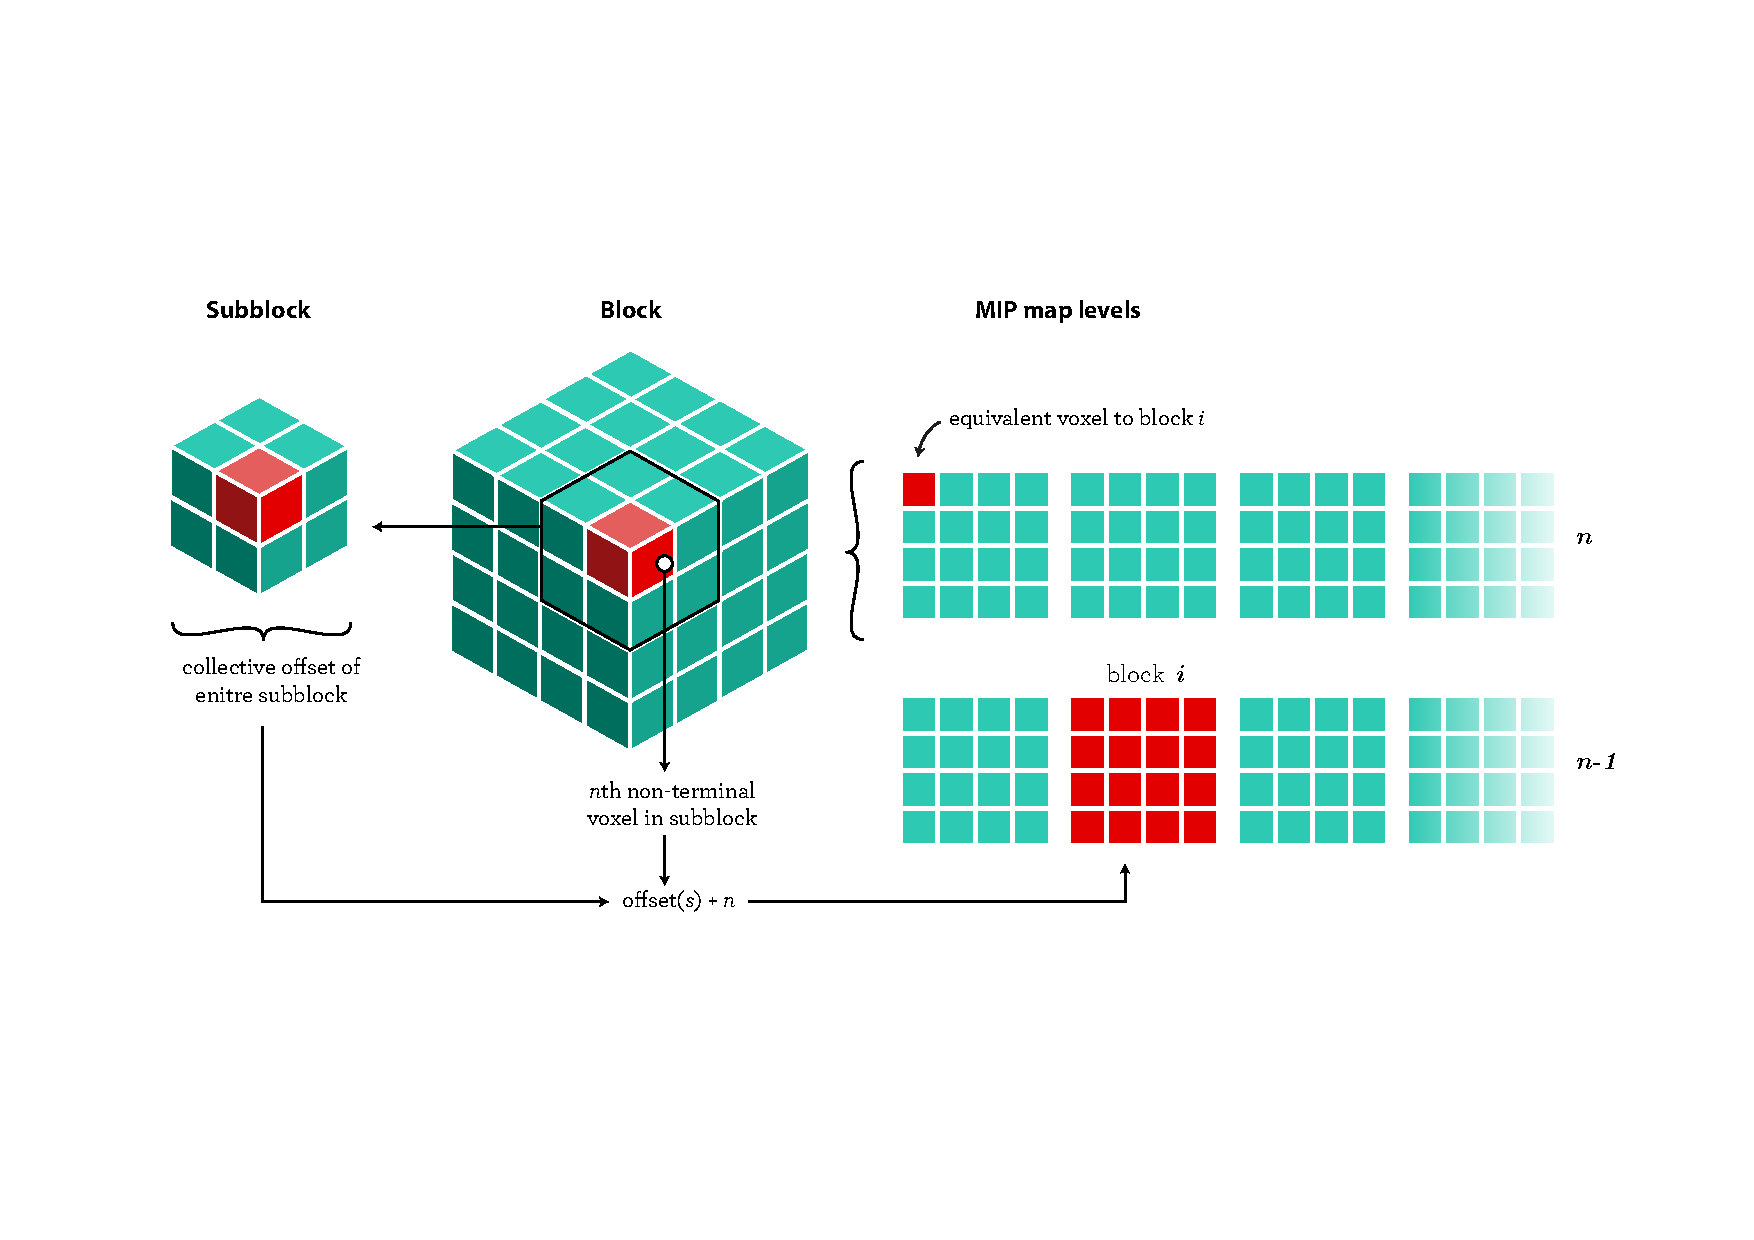
\includegraphics[scale=0.65]{figures/subblock.pdf} 
\caption{Subblock used to store offsets}
\label{fig:subblock}
\end{center}
\end{figure*}

\subsection{Encoding a level}
Encoding can be described top-down: from the entire process, to a per-level basis and finally to the block level. See Figure \ref{fig:encoder} for a block diagram of the simplified algorithm. The input for the encoder is a voxelmap $V_0$ and its output a set of mipmap levels $\{L_0,L_1,\dotsc,L_{n-1}\}$.  The user specifies values for $w$, $r$ and $\delta$. $V_0$ is the original volume and has a \emph{size} and a \emph{type}. The first level that is encoded is therefore the base level $L_0$. The subroutine \texttt{EncodeLevel} takes a voxelmap $V_i$ and returns a sequence of blocks that make up the level $L_i$, and a new voxelmap $V_{i+1}$. $V_{i+1}$ is a \emph{temporary} voxelmap that is $w$ times smaller along each axis than the input $V_{i}$. $V_{i+1}$ is also $w^{i+1}$ times smaller than $V_0$, this number is the \emph{mipmap factor} and is stored in the level's header. $V_{0} \dots V_{n-1}$ are encoded recursively until the width of a certain $V_{n-1}$ is equal or smaller than $r$. This means that there are only $L_{n-2}$ levels generated. The root level, $L_{n-1}$, is simply a level consisting of one block, namely $V_{n-1}$. 

\begin{figure}[b!]
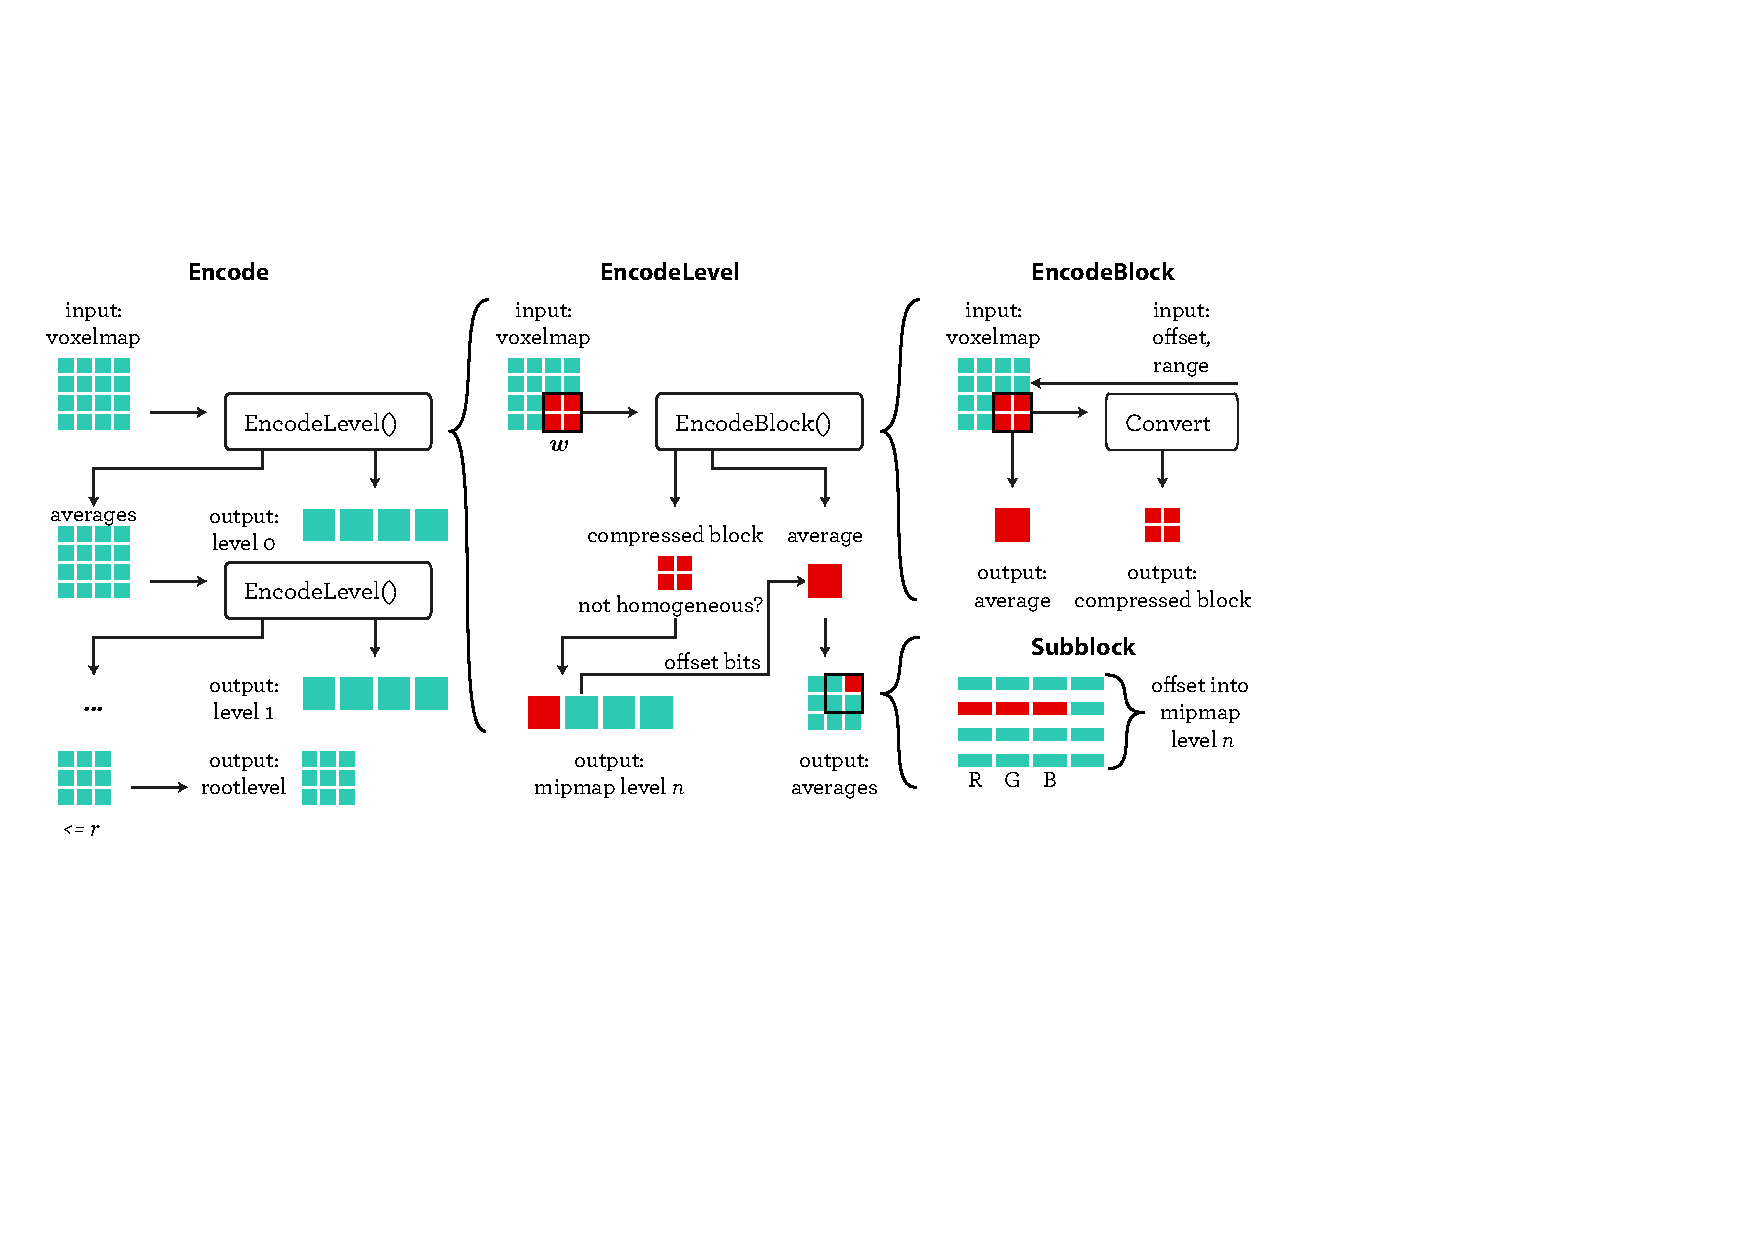
\includegraphics[scale=0.8]{figures/encoder.pdf} 
\caption{Block diagram of the encoder}
\label{fig:encoder}
\end{figure}
%
\subsection{Encoding a block} \label{sec:encodeblock}
%
A level $L_i$ is a sequence of blocks $<B_0,\dotsc,B_{K-1}>$, while a block itself is again a voxelmap of a certain type. Before blocks can be written, the input voxelmap $V_i$ must be a multiple of $w$ and a multiple of 2. Necessary padding will be added. $V_i$ will then be divided into blocks $<B_0,\dotsc,B_{L-1}>$ which are mapped onto the sequence of blocks $<B'_O,\dotsc,B'_{K-1}>$. Note that $K$ and $L$ may or may not be equal. The subroutine \texttt{EncodeBlock} takes a certain input block $B_l$ and an output block $B'_k$. The average $\pmb{\alpha}$ of all voxels in $B_l$ is computed. If $B_l$ is \emph{not} homogeneous, , it is converted, compressed and written to $B'_k$. 

Both compression steps (the $\delta$-parameter and block compression) are applied during the \texttt{EncodeBlock} step. First of all, the $\delta$-parameter is applied during the test for homogeneity. We have empirically determined that using the \emph{vector distance} $ | \pmb{\alpha} - \mathbf{v}_i | $ between the block average $\pmb{\alpha}$ and each individual voxel $\mathbf{v}_i$ in the block, is a good measure for homogeneity. Both the average and the individual voxel are therefore defined as vectors of the voxel's attributes $<a_0,a_1,\dotsc,a_{n-1}$. Homogeneity is now defined as follows:
\begin{align*}
    \mathbf{v}_i &= B_l[i] \\
    \mathrm{homogeneous}(B_l) &= \forall_j : 0 \leq j < size(B_l) : \sqrt{ (\alpha[0] - v_j[0])^2 + \dots + (\alpha[n-1] - v_j[n-1])^2 } \leq \delta \land \mathrm{terminal}(v_j)
\end{align*}

For non-base levels, in order to produce correct subblocks, the conversion of blocks as described above, is performed in groups of $2^3$. Starting at block $B_l$, the resulting set of 8 averages $\{\alpha_l, \dotsc, \alpha_{l+7}\}$ become the equivalent voxels that correspond to the blocks of the sequence $B'_k, \dotsc, B'_{k+7}$ that are not homogeneous. In order to do so, these averages will make up the subblock in $V_{i+1}$ starting at $V_{i+1}[l]$. Furthermore, the offset $o$ of the first non-homogeneous block of the sequence $B'_k, \dotsc, B'_{k+7}$ must be determined (if any). The individual voxels $\{v_l, \dotsc, v_{l+7}\}$ from the subblock $V_{i+1}[l]$ will then be set according to ($<m-n>$ denoting an assignment to selective bits):
\begin{align*}
\forall_i : 0 \leq i < 8 : & \ \\
v_{l+i}<31-8> \ &:= \ \alpha_{l+i}<31-8> & \text{Assign color} \\
v_{l+i}<7-5> \ &:= \ \alpha_{l+i}<7-1> / \ 255 \times 8 & \text{Assign alpha} \\
v_{l+i}<3-0> \ &:= \ o \ \& \ \mathtt{0xf} << 6i & \text{Assign a 4 bit part of the offset } \\
\mathrm{terminal}(v_{l+i}) \ \  &\textit{iff} \ \ \mathrm{homogenous}(B_{l+i}) & \text{Set terminal equiv. voxels}
\end{align*}

For the base level, no terminal flags need to be set. However, block compression can optionally be applied to the non-homogeneous blocks. 


%\end{multicols}

\newcommand{\VEC}[1]{\overline{\mathtt{#1}}}

\iffalse
\begin{algorithm}
\begin{lstlisting}
    $\textit{current position in memory}$
ptr data
    $\textit{either the original voxelmap or the temporary data from the previous level}$
voxelmap $v$ 
    $\textit{width of a block}$
$w$
function EncodeLevel
    vec3 block_count := nextMipmapSize($v$.size,$w$)    
    voxelmap parent := voxelmapCreate($v$.size)
    level_offset := 0
    for $(x,y,z)$ in block_count $/2$ do
        blockgroup_level_offset := level_offset
        for $(i,j,k)$ in vec3$(2,2,2)$ do
            $\textit{Calculate the offset into the given voxelmap}$
            vec3 offset := $(2x+i,2y+j,2z+k)$
            block := EncodeBlock( $v$, offset$*w$ )
            
            voxel := average( block )
            ivec3 subblock_offset := (i,j,k)
            write_offset_part( voxel, subblock_offset, blockgroup_offset )
            
            parent$[offset]$ := average( block )            
            
            if not homogenous( block ) then
                write block at data
                data := data + block_size$(w)$
                level_offset := level_offset + 1;
            fi
        od
    od
end
\end{lstlisting}
\caption{EncodeLevel}
\label{algo:encodelevel}
\end{algorithm}
\fi

